\section{Date: 2026-07-24}
\noindent \textbf{Series ID: BOPGA} 

\noindent This series is titled Unilateral Transfers, Net (DISCONTINUED) and has a frequency of Annual. The units are Billions of Dollars and the seasonal adjustment is Not Seasonally Adjusted.The observation start date is 1960-01-01 and the observation end date is 2013-01-01.The popularity of this series is 1. \\ 

\noindent \textbf{Series ID: BKTTPAA641N} 

\noindent This series is titled Failures and Assistance Transactions of all Institutions by Transaction Type (Purchase and Assumption (PA)) for the United States and Other Areas and has a frequency of Annual. The units are Number of Institutions and the seasonal adjustment is Not Seasonally Adjusted.The observation start date is 1934-01-01 and the observation end date is 2026-01-01.The popularity of this series is 1. \\ 

\subsection{Raw Regression}
\noindent Regresses the two series against each other directly. A significant result here can come just as easily from both series sharing a long-run trend as from any real relationship.

\begin{center}
\begin{tabular}{lclc}
\toprule
\textbf{Dep. Variable:}     & value\_fred\_BKTTPAA641N & \textbf{  R-squared:         } &     0.005   \\
\textbf{Model:}             &           OLS            & \textbf{  Adj. R-squared:    } &    -0.014   \\
\textbf{Method:}            &      Least Squares       & \textbf{  F-statistic:       } &    0.2713   \\
\textbf{Date:}              &     Fri, 24 Jul 2026     & \textbf{  Prob (F-statistic):} &    0.605    \\
\textbf{Time:}              &         13:12:01         & \textbf{  Log-Likelihood:    } &   -308.19   \\
\textbf{No. Observations:}  &              54          & \textbf{  AIC:               } &     620.4   \\
\textbf{Df Residuals:}      &              52          & \textbf{  BIC:               } &     624.4   \\
\textbf{Df Model:}          &               1          & \textbf{                     } &             \\
\textbf{Covariance Type:}   &        nonrobust         & \textbf{                     } &             \\
\bottomrule
\end{tabular}
\begin{tabular}{lcccccc}
                            & \textbf{coef} & \textbf{std err} & \textbf{t} & \textbf{P$> |$t$|$} & \textbf{[0.025} & \textbf{0.975]}  \\
\midrule
\textbf{const}              &      33.0760  &       13.835     &     2.391  &         0.020        &        5.313    &       60.839     \\
\textbf{value\_fred\_BOPGA} &      -0.1284  &        0.247     &    -0.521  &         0.605        &       -0.623    &        0.366     \\
\bottomrule
\end{tabular}
\begin{tabular}{lclc}
\textbf{Omnibus:}       & 41.852 & \textbf{  Durbin-Watson:     } &    0.265  \\
\textbf{Prob(Omnibus):} &  0.000 & \textbf{  Jarque-Bera (JB):  } &  110.404  \\
\textbf{Skew:}          &  2.369 & \textbf{  Prob(JB):          } & 1.06e-24  \\
\textbf{Kurtosis:}      &  8.160 & \textbf{  Cond. No.          } &     76.9  \\
\bottomrule
\end{tabular}
%\caption{OLS Regression Results}
\end{center}

Notes: \newline
 [1] Standard Errors assume that the covariance matrix of the errors is correctly specified.

\begin{figure}
\centering
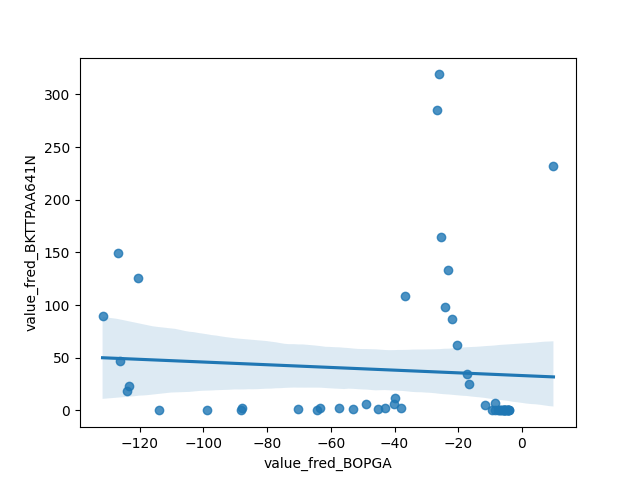
\includegraphics[scale = 0.9]{plots/plot_2026-07-24.png}
\caption{Raw Regression Plot for 2026-07-24}
\end{figure}
\newpage
\subsection{Detrended Regression}
\noindent Regresses the residuals of each series after removing its own linear time trend, so a shared trend can no longer drive the result on its own. A relationship that stays significant here is better evidence of a genuine link between the two series.

\begin{center}
\begin{tabular}{lclc}
\toprule
\textbf{Dep. Variable:}                & value\_fred\_BKTTPAA641N\_detrended & \textbf{  R-squared:         } &     0.085   \\
\textbf{Model:}                        &                 OLS                 & \textbf{  Adj. R-squared:    } &     0.068   \\
\textbf{Method:}                       &            Least Squares            & \textbf{  F-statistic:       } &     4.844   \\
\textbf{Date:}                         &           Fri, 24 Jul 2026          & \textbf{  Prob (F-statistic):} &   0.0322    \\
\textbf{Time:}                         &               13:12:01              & \textbf{  Log-Likelihood:    } &   -304.45   \\
\textbf{No. Observations:}             &                    54               & \textbf{  AIC:               } &     612.9   \\
\textbf{Df Residuals:}                 &                    52               & \textbf{  BIC:               } &     616.9   \\
\textbf{Df Model:}                     &                     1               & \textbf{                     } &             \\
\textbf{Covariance Type:}              &              nonrobust              & \textbf{                     } &             \\
\bottomrule
\end{tabular}
\begin{tabular}{lcccccc}
                                       & \textbf{coef} & \textbf{std err} & \textbf{t} & \textbf{P$> |$t$|$} & \textbf{[0.025} & \textbf{0.975]}  \\
\midrule
\textbf{const}                         &   -2.402e-12  &        9.425     & -2.55e-13  &         1.000        &      -18.912    &       18.912     \\
\textbf{value\_fred\_BOPGA\_detrended} &       1.0857  &        0.493     &     2.201  &         0.032        &        0.096    &        2.076     \\
\bottomrule
\end{tabular}
\begin{tabular}{lclc}
\textbf{Omnibus:}       & 31.844 & \textbf{  Durbin-Watson:     } &    0.291  \\
\textbf{Prob(Omnibus):} &  0.000 & \textbf{  Jarque-Bera (JB):  } &   64.227  \\
\textbf{Skew:}          &  1.865 & \textbf{  Prob(JB):          } & 1.13e-14  \\
\textbf{Kurtosis:}      &  6.825 & \textbf{  Cond. No.          } &     19.1  \\
\bottomrule
\end{tabular}
%\caption{OLS Regression Results}
\end{center}

Notes: \newline
 [1] Standard Errors assume that the covariance matrix of the errors is correctly specified.

\begin{figure}
\centering
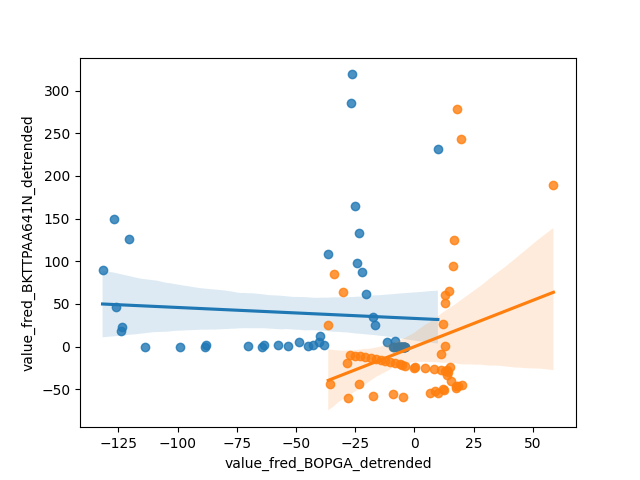
\includegraphics[scale = 0.9]{plots/plot_2026-07-24_detrended.png}
\caption{Detrended Regression Plot for 2026-07-24}
\end{figure}
\newpage
